% Source: AESP_466_ClassWork/Assignments/Assignment_2/AESP466_HW2_Reference_Sp26.tex
% Description: NACA 2412 airfoil showing the outer surface (solid blue), mean camber line (dashed red), and chord reference (gray).

\documentclass[border=4pt]{standalone}
\usepackage{amsmath}
\usepackage{amssymb}
\usepackage{graphicx}
\usepackage{pgfplots}
\usepackage{tikz}
\usepackage{xcolor}
\pgfplotsset{compat=1.18}
\usetikzlibrary{arrows.meta, calc, positioning}

\definecolor{Garnet}{HTML}{73000A}
\definecolor{USC_Rose}{HTML}{CC2E40}
\definecolor{USC_Blue}{HTML}{466A9F}
\definecolor{USC_Slate}{HTML}{1F414D}
\definecolor{USC_Olive}{HTML}{65780B}
\definecolor{USC_Lime}{HTML}{CED318}
\definecolor{USC_Gold}{HTML}{A49137}
\definecolor{USC_Black90}{HTML}{565656}
\definecolor{USC_Black10}{HTML}{ECECEC}


\begin{document}
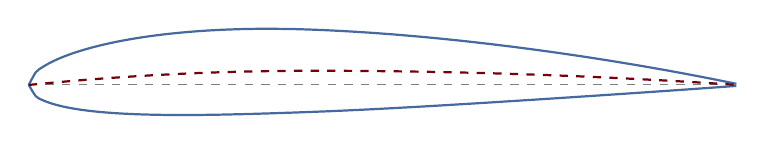
\begin{tikzpicture}[scale=9]
    \draw[dashed, gray] (0,0) -- (1,0);
    \def\m{0.02}
    \def\p{0.4}
    \def\th{0.12}
    \draw[thick, USC_Blue, domain=0:1, samples=100, smooth] plot (\x, {
        (\th/0.2)*(0.2969*sqrt(\x) - 0.1260*\x - 0.3516*\x^2 + 0.2843*\x^3 - 0.1015*\x^4) +
        (\x < \p ? (\m/(\p*\p))*(2*\p*\x - \x*\x) : (\m/((1-\p)*(1-\p)))*((1-2*\p)+2*\p*\x-\x*\x))
    });
    \draw[thick, USC_Blue, domain=0:1, samples=100, smooth] plot (\x, {
        -1*(\th/0.2)*(0.2969*sqrt(\x) - 0.1260*\x - 0.3516*\x^2 + 0.2843*\x^3 - 0.1015*\x^4) +
        (\x < \p ? (\m/(\p*\p))*(2*\p*\x - \x*\x) : (\m/((1-\p)*(1-\p)))*((1-2*\p)+2*\p*\x-\x*\x))
    });
    \draw[Garnet, thick, dashed, domain=0:1, samples=50] plot (\x, {
        (\x < \p ? (\m/(\p*\p))*(2*\p*\x - \x*\x) : (\m/((1-\p)*(1-\p)))*((1-2*\p)+2*\p*\x-\x*\x))
    });
\end{tikzpicture}
\end{document}
